\documentclass[fontsize=7.5pt,twoside]{scrartcl}
\usepackage[paperwidth=70mm,paperheight=90mm,inner=7.5mm,outer=4mm,
  top=8mm,bottom=7mm,headheight=9pt,headsep=2.2mm,footskip=4mm]{geometry}
\usepackage{fontspec}
\usepackage{polyglossia}
\setdefaultlanguage{russian}
\setmainfont{Inter}[BoldFont={Inter Bold}]
\setsansfont{Inter}[BoldFont={Inter Bold}]
\newfontfamily\cyrillicfont{Inter}[BoldFont={Inter Bold}]
\newfontfamily\cyrillicfontsf{Inter}[BoldFont={Inter Bold}]
\usepackage{amsmath}
\usepackage{unicode-math}
\setmathfont{Latin Modern Math}
\usepackage{icomma}
\usepackage{enumitem}
\usepackage{fancyhdr}
\usepackage{array}
\usepackage{tikz}
\usetikzlibrary{angles,quotes,calc,decorations.pathreplacing}
\usepackage[most]{tcolorbox}

\linespread{1.08}
\setlength{\parindent}{0pt}
\setlength{\parskip}{0.6pt}
\raggedright
\addtokomafont{disposition}{\rmfamily}

% ---------- колонтитулы ----------
\newcommand{\taskhead}{}
\pagestyle{fancy}
\fancyhf{}
\fancyhead[LE]{\footnotesize\bfseries\taskhead}
\fancyhead[RO]{\footnotesize\bfseries\taskhead}
\fancyfoot[LE,RO]{\footnotesize\bfseries\thepage}
\renewcommand{\headrulewidth}{0.6pt}

% ---------- визуальный код (ч/б) ----------
\tcbset{boxsep=0pt,left=1.2mm,right=1.2mm,top=0.9mm,bottom=0.9mm,
  arc=0.8mm,before skip=1.3mm,after skip=1.3mm,before upper=\raggedright}
% формулы: сплошная рамка
\newtcolorbox{fbx}{enhanced,colback=white,colframe=black,boxrule=0.6pt}
% ловушки: пунктирная рамка + «!»
\newtcolorbox{trap}{enhanced,colback=white,frame hidden,
  borderline={0.6pt}{0pt}{black,dash pattern=on 1.6pt off 1.1pt}}
% пример: серая заливка 18 %
\newtcolorbox{ex}{enhanced,colback=black!18,frame hidden}

\newcommand{\warn}{\tikz[baseline=-0.65ex]\node[circle,draw,line width=0.6pt,
  inner sep=0.5pt,minimum size=2.6mm,font=\bfseries\scriptsize]{!};\ }
\newcommand{\blk}[1]{\par\smallskip{\bfseries\MakeUppercase{#1}}\par\nopagebreak\smallskip}
\setlist{nosep,leftmargin=3mm,labelsep=1mm}
\setlist[itemize]{label=–}
\setlist[enumerate]{label=\bfseries\arabic*.}

\newcommand{\task}[2]{\renewcommand{\taskhead}{Задание #1 · #2}}
\newcommand{\tpage}[2]{%
  {\Large\bfseries Задание #1\par}\smallskip
  {\large\bfseries #2\par}\medskip\hrule height 0.6pt\medskip}
\newcommand{\pg}[1]{\dotfill\,#1}

% ---------- чертежи ----------
\tikzset{every picture/.append style={line width=0.5pt},
  hid/.style={dash pattern=on 1.4pt off 1pt},
  lb/.style={font=\scriptsize},
  sh/.style={fill=black!18}}
\newcommand{\fig}[1]{\par\smallskip{\centering #1\par}\smallskip}
% куб: x0,y0,a
\newcommand{\cube}[3]{\begin{scope}[shift={(#1,#2)}]
 \draw (0,0) rectangle (#3,#3);
 \draw (0,#3)--++({0.4*#3},{0.3*#3})--++(#3,0)--(#3,#3);
 \draw ({1.4*#3},{1.3*#3})--++(0,-#3)--(#3,0);
 \draw[hid] (0,0)--++({0.4*#3},{0.3*#3})--++(#3,0) ({0.4*#3},{0.3*#3})--++(0,#3);
 \end{scope}}
% цилиндр: x0,R,H,уровень жидкости (0 — нет)
\newcommand{\cyl}[4]{\begin{scope}[shift={(#1,0)}]
 \ifdim #4pt>0pt
 \fill[black!18] (-#2,0) arc[start angle=180,end angle=360,x radius=#2,y radius={0.25*#2}]
   --(#2,#4) arc[start angle=0,end angle=-180,x radius=#2,y radius={0.25*#2}]--cycle;
 \fill[black!18] (0,#4) ellipse[x radius=#2,y radius={0.25*#2}];
 \draw (0,#4) ellipse[x radius=#2,y radius={0.25*#2}];
 \fi
 \draw (-#2,0) arc[start angle=180,end angle=360,x radius=#2,y radius={0.25*#2}];
 \draw[hid] (#2,0) arc[start angle=0,end angle=180,x radius=#2,y radius={0.25*#2}];
 \draw (0,#3) ellipse[x radius=#2,y radius={0.25*#2}];
 \draw (-#2,0)--(-#2,#3) (#2,0)--(#2,#3);
 \end{scope}}
% конус: R,H
\newcommand{\cone}[2]{%
 \draw (-#1,0) arc[start angle=180,end angle=360,x radius=#1,y radius={0.25*#1}];
 \draw[hid] (#1,0) arc[start angle=0,end angle=180,x radius=#1,y radius={0.25*#1}];
 \draw (-#1,0)--(0,#2)--(#1,0);}
% шар: R
\newcommand{\ball}[1]{%
 \draw (0,0) circle (#1);
 \draw (-#1,0) arc[start angle=180,end angle=360,x radius=#1,y radius={0.25*#1}];
 \draw[hid] (#1,0) arc[start angle=0,end angle=180,x radius=#1,y radius={0.25*#1}];}
% правильная четырёхугольная пирамида
\newcommand{\pyr}[1]{%
 \coordinate (A) at (0,0); \coordinate (B) at (2.6,0); \coordinate (C) at (3.4,0.7);
 \coordinate (D) at (0.8,0.7); \coordinate (O) at (1.7,0.35); \coordinate (S) at (1.7,2.5);
 \coordinate (K) at (1.3,0);
 #1
 \draw (A)--(B)--(C)--(S)--cycle (S)--(B);
 \draw[hid] (A)--(D)--(C) (D)--(S) (S)--(O);
 \fill (O) circle (0.035);}
% вектор
\tikzset{vec/.style={-{Stealth[length=1.6mm]},line width=0.6pt}}
\usetikzlibrary{arrows.meta}
% оси
\newcommand{\axes}[4]{\draw[-{Stealth[length=1.3mm]}] (#1,0)--(#2,0) node[right,lb]{$x$};
 \draw[-{Stealth[length=1.3mm]}] (0,#3)--(0,#4) node[above,lb]{$y$};
 \node[below left,lb] at (0,0) {$O$};}
\newcommand{\proto}[2]{{\bfseries ПРОТОТИП #1\par}{\footnotesize #2\par}\smallskip}
\newcommand{\sol}{\par\smallskip\textbf{Решение.}\ }
\newcommand{\ans}[1]{\par\smallskip\textbf{Ответ:} #1\par}
% стандартный треугольник для теории
\newcommand{\tri}{\coordinate (A) at (0,0); \coordinate (B) at (1.2,2); \coordinate (C) at (4,0);
 \draw (A)--(B)--(C)--cycle;
 \node[below left,lb] at (A){$A$}; \node[above,lb] at (B){$B$}; \node[below right,lb] at (C){$C$};}
\begin{document}
\setcounter{page}{12}

%==================== ЗАДАНИЕ 1 ====================
\task{1}{Планиметрия}
\tpage{1}{Планиметрия}
\blk{Что спрашивают}
Угол, длину, площадь или синус (косинус) угла плоской фигуры.
\blk{Алгоритм}
\begin{enumerate}
\item Нарисуй чертёж, отметь данные и искомое.
\item Назови фигуру, вспомни её свойства (с.~13–23).
\item Ищи прямоугольный или равнобедренный треугольник. Нет его~— проведи радиус в~точку касания или высоту.
\item Запиши формулу, подставь числа.
\item Проверь: углы треугольника в~сумме $180^\circ$, синус и~косинус острого угла меньше~1.
\end{enumerate}
\blk{В бланк}
Число, без единиц и~знака градуса: \textbf{2,5}.

\newpage %13
\blk{Углы и параллельные прямые}
\fig{\begin{tikzpicture}[scale=0.82]
\coordinate (Pb) at (1.8,0); \coordinate (Pa) at (2.724,1.6);
\draw (0,0)--(5,0) node[right,lb]{$b$};
\draw (0,1.6)--(5,1.6) node[right,lb]{$a$};
\draw ($(Pb)+(240:0.75)$)--($(Pa)+(60:0.75)$) node[right,lb]{$c$};
\foreach \P/\n/\m/\k/\l in {Pa/1/2/3/4, Pb/5/6/7/8}{
 \node[lb] at ($(\P)+(120:0.34)$) {\n};
 \node[lb] at ($(\P)+(30:0.55)$) {\m};
 \node[lb] at ($(\P)+(210:0.55)$) {\k};
 \node[lb] at ($(\P)+(300:0.34)$) {\l};}
\end{tikzpicture}}
\begin{fbx}
Вертикальные равны: $\angle1=\angle4$,\ $\angle2=\angle3$\\
Смежные: $\angle1+\angle2=180^\circ$
\end{fbx}
\begin{fbx}
$a\parallel b$:\\[0.3mm]
Накрест лежащие: $\angle3=\angle6$,\ $\angle4=\angle5$\\
Соответственные: $\angle1=\angle5$,\ $\angle2=\angle6$,\\ \hspace*{3mm}$\angle3=\angle7$,\ $\angle4=\angle8$\\
Односторонние: $\angle3+\angle5=180^\circ$,\\ \hspace*{3mm}$\angle4+\angle6=180^\circ$
\end{fbx}
Обратно: если верно хотя бы одно из этих равенств, то $a\parallel b$.

\newpage %14
\blk{Углы треугольника}
\fig{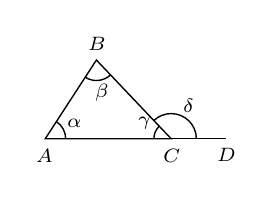
\begin{tikzpicture}[scale=0.5]
\coordinate (A) at (0,0); \coordinate (B) at (1.3,2); \coordinate (C) at (3.2,0); \coordinate (D) at (4.6,0);
\draw (A)--(B)--(C)--cycle; \draw (C)--(D);
\pic[draw,angle radius=2.6mm] {angle=C--A--B};
\pic[draw,angle radius=2.6mm] {angle=A--B--C};
\pic[draw,angle radius=2.2mm] {angle=B--C--A};
\pic[draw,angle radius=3.2mm] {angle=D--C--B};
\node[lb] at ($(A)+(28:0.85)$) {$\alpha$}; \node[lb] at ($(B)+(-80:0.85)$) {$\beta$};
\node[lb] at ($(C)+(150:0.8)$) {$\gamma$}; \node[lb] at ($(C)+(62:0.95)$) {$\delta$};
\node[below,lb] at (A) {$A$}; \node[above,lb] at (B) {$B$}; \node[below,lb] at (C) {$C$}; \node[below,lb] at (D) {$D$};
\end{tikzpicture}\quad
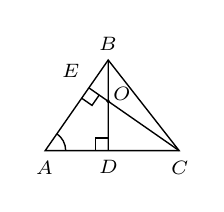
\begin{tikzpicture}[scale=0.5]
\coordinate (A) at (0,0); \coordinate (B) at (1.6,2.3); \coordinate (C) at (3.4,0);
\coordinate (D) at ($(A)!(B)!(C)$); \coordinate (E) at ($(A)!(C)!(B)$);
\coordinate (O) at (intersection of B--D and C--E);
\draw (A)--(B)--(C)--cycle; \draw (B)--(D) (C)--(E);
\pic[draw,angle radius=1.6mm] {right angle=B--D--A};
\pic[draw,angle radius=1.6mm] {right angle=A--E--C};
\pic[draw,angle radius=2.6mm] {angle=C--A--B};
\fill (O) circle (0.05);
\node[below,lb] at (A) {$A$}; \node[above,lb] at (B) {$B$}; \node[below,lb] at (C) {$C$};
\node[below,lb] at (D) {$D$}; \node[above left,lb] at (E) {$E$}; \node[lb] at ($(O)+(27.6:0.4)$) {$O$};
\end{tikzpicture}}
\begin{fbx}
$\alpha+\beta+\gamma=180^\circ$\qquad Внешний: $\delta=\alpha+\beta$
\end{fbx}
\begin{fbx}
Четырёхугольник: $360^\circ$;\ $n$-угольник: $180^\circ(n-2)$\\[0.4mm]
Высоты $BD$, $CE$: в $ADOE$ $\angle D=\angle E=90^\circ\Rightarrow$\\
$\angle DOE=180^\circ-\angle A$
\end{fbx}
\fig{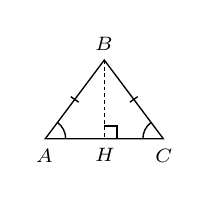
\begin{tikzpicture}[scale=0.5]
\coordinate (A) at (0,0); \coordinate (B) at (1.5,2); \coordinate (C) at (3,0); \coordinate (H) at (1.5,0);
\draw (A)--(B)--(C)--cycle; \draw[hid] (B)--(H);
\pic[draw,angle radius=1.6mm] {right angle=B--H--C};
\pic[draw,angle radius=2.6mm] {angle=C--A--B}; \pic[draw,angle radius=2.6mm] {angle=B--C--A};
\draw ($(A)!0.5!(B)+(-0.1,0.07)$)--++(0.2,-0.14); \draw ($(B)!0.5!(C)+(-0.1,-0.07)$)--++(0.2,0.14);
\node[below,lb] at (A) {$A$}; \node[above,lb] at (B) {$B$}; \node[below,lb] at (C) {$C$}; \node[below,lb] at (H) {$H$};
\end{tikzpicture}}
\begin{fbx}
$AB=BC\Rightarrow\angle A=\angle C$;\ $BH$~— медиана, биссектриса и~высота
\end{fbx}

\newpage %15
\blk{Медиана, средняя линия, биссектриса}
\fig{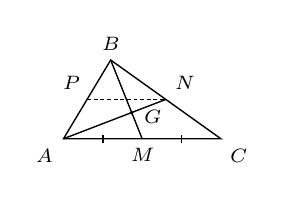
\begin{tikzpicture}[scale=0.5]
\tri
\coordinate (M) at (2,0); \coordinate (P) at (0.6,1); \coordinate (N) at (2.6,1);
\draw (B)--(M); \draw (A)--(N); \draw[hid] (P)--(N);
\coordinate (G) at (intersection of B--M and A--N); \fill (G) circle (0.05);
\node[below,lb] at (M){$M$}; \node[above left,lb] at (P){$P$}; \node[above right,lb] at (N){$N$};
\node[right,lb] at ($(G)+(0.08,-0.12)$) {$G$};
\draw (1,-0.1)--(1,0.1) (3,-0.1)--(3,0.1);
\end{tikzpicture}}
\begin{fbx}
\textbf{Медиана} $BM$ делит площадь пополам.\\
Медианы $BM$, $AN$ пересекаются в $G$:\ $BG:GM=2:1$\\[0.4mm]
\textbf{Средняя линия} $PN\parallel AC$,\ $PN=\tfrac12\,AC$
\end{fbx}
\fig{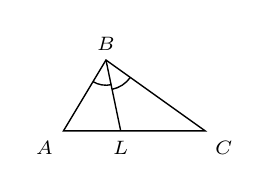
\begin{tikzpicture}[scale=0.45]
\tri
\coordinate (L) at (1.616,0); \draw (B)--(L); \node[below,lb] at (L){$L$};
\pic[draw,angle radius=3.2mm] {angle=A--B--L};
\pic[draw,angle radius=3.8mm] {angle=L--B--C};
\end{tikzpicture}}
\begin{fbx}
\textbf{Биссектриса} $BL$:\ \ $\dfrac{AL}{LC}=\dfrac{AB}{BC}$
\end{fbx}

\newpage %16
\blk{Площадь треугольника}
\fig{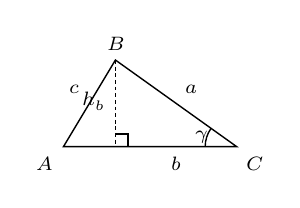
\begin{tikzpicture}[scale=0.55]
\tri
\coordinate (H) at (1.2,0);
\draw[hid] (B)--(H); \pic[draw,angle radius=1.6mm] {right angle=B--H--C};
\node[left,lb] at (1.2,1.05){$h_b$};
\node[below,lb] at (2.6,0){$b$}; \node[above right,lb] at (2.6,1){$a$}; \node[above left,lb] at (0.6,1){$c$};
\pic[draw,angle radius=4mm] {angle=B--C--A}; \node[lb] at ($(C)+(165:0.85)$) {$\gamma$};
\end{tikzpicture}}
\begin{fbx}
$S=\tfrac12\,b\,h_b$\qquad $S=\tfrac12\,ab\sin\gamma$
\end{fbx}
\begin{fbx}
$S=\sqrt{p(p-a)(p-b)(p-c)}$,\ \ $p=\dfrac{a+b+c}{2}$
\end{fbx}
\fig{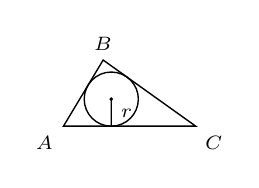
\begin{tikzpicture}[scale=0.42]
\tri
\coordinate (I) at (1.4457,0.8186); \draw (I) circle (0.8186); \fill (I) circle (0.06);
\draw (I)--(1.4457,0); \node[right,lb] at (1.4457,0.38) {$r$};
\end{tikzpicture}\quad
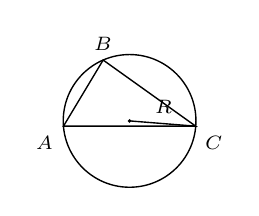
\begin{tikzpicture}[scale=0.42]
\tri
\coordinate (O) at (2,0.16); \draw (O) circle (2.0064); \fill (O) circle (0.06);
\draw (O)--(C); \node[above,lb] at (3.05,0.08) {$R$};
\end{tikzpicture}}
\begin{fbx}
$S=p\,r$\qquad $S=\dfrac{abc}{4R}$
\end{fbx}

\newpage %17
\fig{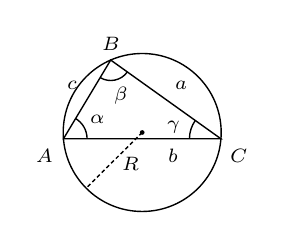
\begin{tikzpicture}[scale=0.5]
\tri
\coordinate (O) at (2,0.16); \draw (O) circle (2.0064); \fill (O) circle (0.06);
\draw[hid] (O)--(0.58,-1.25); \node[right,lb] at (1.25,-0.65) {$R$};
\node[above right,lb] at (2.6,1){$a$}; \node[below,lb] at (2.8,0){$b$}; \node[above left,lb] at (0.6,1){$c$};
\pic[draw,angle radius=3mm] {angle=C--A--B};
\pic[draw,angle radius=2.6mm] {angle=A--B--C};
\pic[draw,angle radius=4mm] {angle=B--C--A};
\node[lb] at ($(A)+(29.5:1.0)$) {$\alpha$}; \node[lb] at ($(B)+(-74:0.95)$) {$\beta$}; \node[lb] at ($(C)+(166.7:1.25)$) {$\gamma$};
\end{tikzpicture}\quad
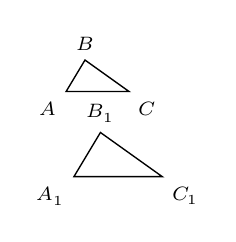
\begin{tikzpicture}[scale=0.2]
\tri
\begin{scope}[shift={(0.5,-5.4)},scale=1.4]
\coordinate (A1) at (0,0); \coordinate (B1) at (1.2,2); \coordinate (C1) at (4,0);
\draw (A1)--(B1)--(C1)--cycle;
\node[below left,lb] at (A1){$A_1$}; \node[above,lb] at (B1){$B_1$}; \node[below right,lb] at (C1){$C_1$};
\end{scope}
\end{tikzpicture}}
\blk{Теорема синусов и косинусов}
\begin{fbx}
$\dfrac{a}{\sin\alpha}=\dfrac{b}{\sin\beta}=\dfrac{c}{\sin\gamma}=2R$\\[0.6mm]
$c^2=a^2+b^2-2ab\cos\gamma$
\end{fbx}
\begin{fbx}
$\sin(180^\circ-\alpha)=\sin\alpha$,\ $\cos(180^\circ-\alpha)=-\cos\alpha$\\[0.3mm]
$\sin120^\circ=\tfrac{\sqrt3}{2}$,\ $\sin135^\circ=\tfrac{\sqrt2}{2}$,\ $\sin150^\circ=\tfrac12$
\end{fbx}
\begin{fbx}
\textbf{Подобие}, $k=\tfrac{A_1B_1}{AB}$:\\ длины $\times k$, площади $\times k^2$\\[0.3mm]
Признаки: два угла; две стороны и~угол между ними; три стороны
\end{fbx}

\newpage %18
\blk{Прямоугольный треугольник}
\fig{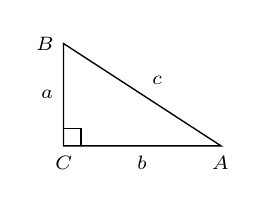
\begin{tikzpicture}[scale=0.5]
\coordinate (C) at (0,0); \coordinate (A) at (4,0); \coordinate (B) at (0,2.6);
\draw (C)--(A)--(B)--cycle;
\pic[draw,angle radius=2.2mm] {right angle=A--C--B};
\node[below,lb] at (C) {$C$}; \node[below,lb] at (A) {$A$}; \node[left,lb] at (B) {$B$};
\node[below,lb] at (2,0) {$b$}; \node[left,lb] at (0,1.3) {$a$};
\node[above right,lb] at (2,1.3) {$c$};
\end{tikzpicture}}
\begin{fbx}
$c^2=a^2+b^2$\\[0.6mm]
$\sin A=\dfrac{a}{c}$\quad $\cos A=\dfrac{b}{c}$\quad $\operatorname{tg}A=\dfrac{a}{b}=\dfrac{\sin A}{\cos A}$\\[0.6mm]
$\sin^2A+\cos^2A=1$
\end{fbx}
\fig{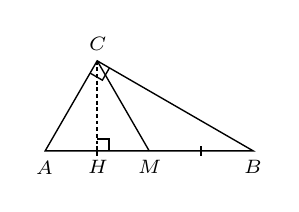
\begin{tikzpicture}[scale=0.6]
\coordinate (A) at (0,0); \coordinate (B) at (4.4,0); \coordinate (C) at (1.1,1.905);
\coordinate (M) at (2.2,0); \coordinate (H) at (1.1,0);
\draw (A)--(B)--(C)--cycle; \draw (C)--(M); \draw[hid] (C)--(H);
\pic[draw,angle radius=1.8mm] {right angle=A--C--B};
\pic[draw,angle radius=1.5mm] {right angle=C--H--B};
\draw (1.1,-0.1)--(1.1,0.1) (3.3,-0.1)--(3.3,0.1);
\node[below,lb] at (A) {$A$}; \node[below,lb] at (B) {$B$}; \node[above,lb] at (C) {$C$};
\node[below,lb] at (M) {$M$}; \node[below,lb] at (H) {$H$};
\end{tikzpicture}}
\begin{fbx}
$CM=AM=BM=\tfrac c2=R\ \Rightarrow\ \angle ACM=\angle A$\\[0.4mm]
Высота: $\angle ACH=90^\circ-\angle A=\angle B$
\end{fbx}

\newpage %19
\blk{Ещё о прямоугольном}
\fig{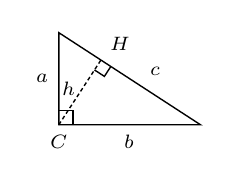
\begin{tikzpicture}[scale=0.45]
\coordinate (C) at (0,0); \coordinate (A) at (4,0); \coordinate (B) at (0,2.6);
\draw (C)--(A)--(B)--cycle;
\pic[draw,angle radius=1.8mm] {right angle=A--C--B};
\coordinate (H) at ($(A)!(C)!(B)$); \draw[hid] (C)--(H);
\pic[draw,angle radius=1.5mm] {right angle=C--H--A};
\node[lb] at (0.3,1.0) {$h$};
\node[below,lb] at (2,0) {$b$}; \node[left,lb] at (0,1.3) {$a$};
\node[above right,lb] at (2.3,1.1) {$c$};
\node[below,lb] at (C) {$C$}; \node[above right,lb] at (H) {$H$};
\end{tikzpicture}\quad
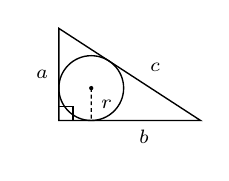
\begin{tikzpicture}[scale=0.45]
\coordinate (C) at (0,0); \coordinate (A) at (4,0); \coordinate (B) at (0,2.6);
\draw (C)--(A)--(B)--cycle;
\pic[draw,angle radius=1.8mm] {right angle=A--C--B};
\coordinate (I) at (0.9146,0.9146); \draw (I) circle (0.9146); \fill (I) circle (0.06);
\draw[hid] (I)--(0.9146,0); \node[right,lb] at (0.9146,0.45) {$r$};
\node[below,lb] at (2.4,0) {$b$}; \node[left,lb] at (0,1.3) {$a$};
\node[above right,lb] at (2.3,1.1) {$c$};
\end{tikzpicture}}
\begin{fbx}
$h=\dfrac{ab}{c}$\qquad $r=\dfrac{a+b-c}{2}$
\end{fbx}
Тройки: $3,4,5$;\ $5,12,13$;\ $8,15,17$;\ $7,24,25$
\renewcommand{\arraystretch}{1.4}
\begin{center}
\begin{tabular}{|c|c|c|c|}
\hline
 & $30^\circ$ & $45^\circ$ & $60^\circ$\\\hline
$\sin$ & $\frac12$ & $\frac{\sqrt2}{2}$ & $\frac{\sqrt3}{2}$\\\hline
$\cos$ & $\frac{\sqrt3}{2}$ & $\frac{\sqrt2}{2}$ & $\frac12$\\\hline
$\operatorname{tg}$ & $\frac{\sqrt3}{3}$ & $1$ & $\sqrt3$\\\hline
\end{tabular}
\end{center}
\begin{fbx}
$\sin30^\circ=\tfrac12$: катет против $30^\circ$ равен $\dfrac c2$
\end{fbx}

\newpage %20
\blk{Параллелограмм}
\fig{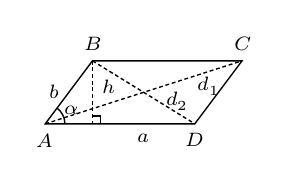
\begin{tikzpicture}[scale=0.5]
\coordinate (A) at (0,0); \coordinate (B) at (1.2,1.6); \coordinate (C) at (5,1.6); \coordinate (D) at (3.8,0);
\draw (A)--(B)--(C)--(D)--cycle; \draw[hid] (A)--(C) (B)--(D);
\draw[hid] (B)--(1.2,0); \draw (1.2,0.2)--(1.4,0.2)--(1.4,0); \node[right,lb] at (1.2,0.95) {$h$};
\node[below,lb] at (2.5,0) {$a$}; \node[left,lb] at (0.6,0.8) {$b$};
\node[lb] at (4.15,0.95) {$d_1$}; \node[lb] at (3.35,0.58) {$d_2$};
\pic[draw,angle radius=2.5mm] {angle=D--A--B};
\node[lb] at ($(A)+(27:0.75)$) {$\alpha$};
\node[below,lb] at (A) {$A$}; \node[above,lb] at (B) {$B$}; \node[above,lb] at (C) {$C$}; \node[below,lb] at (D) {$D$};
\end{tikzpicture}}
Противоположные стороны и углы равны, соседние углы в~сумме $180^\circ$, диагонали делятся пополам.
\begin{fbx}
$S=a\,h=ab\sin\alpha$\qquad $d_1^2+d_2^2=2(a^2+b^2)$
\end{fbx}
\textbf{Прямоугольник:} диагонали равны.
\fig{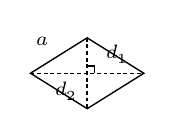
\begin{tikzpicture}[scale=0.45]
\draw (0,0)--(1.6,1)--(3.2,0)--(1.6,-1)--cycle;
\draw[hid] (0,0)--(3.2,0) (1.6,1)--(1.6,-1);
\draw (1.6,0.2)--(1.8,0.2)--(1.8,0);
\node[above,lb] at (2.45,0) {$d_1$}; \node[left,lb] at (1.6,-0.5) {$d_2$};
\node[above left,lb] at (0.8,0.5) {$a$};
\end{tikzpicture}\qquad
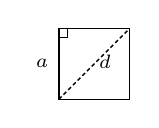
\begin{tikzpicture}[scale=0.45]
\draw (0,-1) rectangle (2,1); \draw[hid] (0,-1)--(2,1);
\node[left,lb] at (0,0) {$a$}; \node[lb] at (1.3,0.05) {$d$};
\draw (0,0.75)--(0.25,0.75)--(0.25,1);
\end{tikzpicture}}
\begin{fbx}
Ромб: $S=\tfrac12\,d_1d_2$,\ $d_1\perp d_2$\\ Квадрат: $d=a\sqrt2$
\end{fbx}

\newpage %21
\blk{Трапеция}
\fig{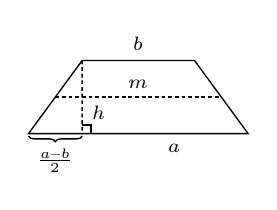
\begin{tikzpicture}[scale=0.62]
\coordinate (A) at (0,0); \coordinate (D) at (4.5,0); \coordinate (C) at (3.4,1.5); \coordinate (B) at (1.1,1.5);
\draw (A)--(B)--(C)--(D)--cycle;
\draw[hid] (0.55,0.75)--(3.95,0.75); \node[above,lb] at (2.25,0.72) {$m$};
\draw[hid] (B)--(1.1,0); \draw (1.1,0.18)--(1.28,0.18)--(1.28,0); \node[right,lb] at (1.1,0.42) {$h$};
\node[above,lb] at (2.25,1.5) {$b$}; \node[below,lb] at (3,0) {$a$};
\draw[decorate,decoration={brace,mirror,amplitude=2pt}] (0,-0.05)--(1.1,-0.05);
\node[below,lb] at (0.55,-0.1) {$\frac{a-b}{2}$};
\end{tikzpicture}}
\begin{fbx}
$m=\dfrac{a+b}{2}$\qquad $S=\dfrac{a+b}{2}\cdot h$
\end{fbx}
\textbf{Равнобедренная:} углы при основании и~диагонали равны; высота отсекает $\dfrac{a-b}{2}$.
\blk{Любой четырёхугольник}
\fig{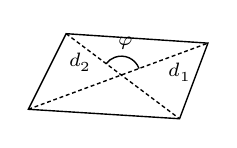
\begin{tikzpicture}[scale=0.6]
\coordinate (P) at (0,0); \coordinate (Q) at (0.8,1.6); \coordinate (R) at (3.8,1.4); \coordinate (T) at (3.2,-0.2);
\draw (P)--(Q)--(R)--(T)--cycle; \draw[hid] (P)--(R) (Q)--(T);
\coordinate (X) at (intersection of P--R and Q--T);
\pic[draw,angle radius=2.4mm] {angle=R--X--Q};
\node[lb] at ($(X)+(81.6:0.68)$) {$\varphi$};
\node[lb] at (3.2,0.78) {$d_1$}; \node[lb] at (1.1,1.0) {$d_2$};
\end{tikzpicture}}
\begin{fbx}
$S=\tfrac12\,d_1d_2\sin\varphi$
\end{fbx}

\newpage %22
\blk{Окружность и углы в ней}
\fig{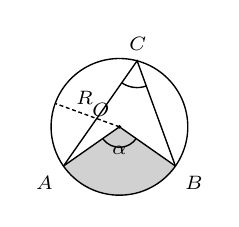
\begin{tikzpicture}[scale=0.62]
\coordinate (O) at (0,0);
\coordinate (A) at (215:1.4); \coordinate (B) at (325:1.4); \coordinate (C) at (75:1.4);
\fill[black!18] (O)--(A) arc[start angle=215,end angle=325,radius=1.4]--cycle;
\draw (O) circle (1.4);
\draw (A)--(O)--(B); \draw (A)--(C)--(B);
\pic[draw,angle radius=2.6mm] {angle=A--O--B}; \node[lb] at (0,-0.48) {$\alpha$};
\pic[draw,angle radius=3.4mm] {angle=A--C--B};
\fill (O) circle (0.04);
\node[above left,lb] at (O) {$O$}; \node[below left,lb] at (A) {$A$};
\node[below right,lb] at (B) {$B$}; \node[above,lb] at (C) {$C$};
\draw[hid] (O)--(160:1.4); \node[above,lb] at (160:0.75) {$R$};
\end{tikzpicture}}
\begin{fbx}
$L=2\pi R$\qquad $S=\pi R^2$\\[0.4mm]
Дуга: $l=\dfrac{\pi R\alpha}{180}$\qquad Сектор: $S=\dfrac{\pi R^2\alpha}{360}$
\end{fbx}
\begin{fbx}
Центральный: $\angle AOB=\cup AB=\alpha$\\
Вписанный: $\angle ACB=\tfrac12\cup AB=\tfrac{\alpha}{2}$
\end{fbx}
\begin{itemize}
\item на одну дугу~— вписанные углы равны;
\item на диаметр~— $90^\circ$;
\item на одну хорду с~разных сторон~— в~сумме $180^\circ$.
\end{itemize}
Центр вписанной окружности~— точка пересечения биссектрис, описанной~— серединных перпендикуляров.

\newpage %23
\blk{Касательная}
\fig{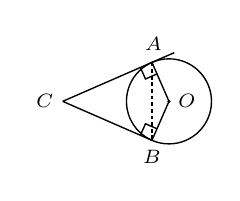
\begin{tikzpicture}[scale=0.45]
\coordinate (O) at (0,0); \coordinate (C) at (-3,0);
\coordinate (A) at (113.58:1.2); \coordinate (B) at (-113.58:1.2);
\draw (O) circle (1.2); \draw (C)--($(C)!1.25!(A)$) (C)--(B);
\draw (O)--(A) (O)--(B); \draw[hid] (A)--(B);
\pic[draw,angle radius=1.6mm] {right angle=C--A--O};
\pic[draw,angle radius=1.6mm] {right angle=O--B--C};
\fill (O) circle (0.05);
\node[right,lb] at (O) {$O$}; \node[left,lb] at (C) {$C$};
\node[above,lb] at ($(A)+(0.05,0.05)$) {$A$}; \node[below,lb] at (B) {$B$};
\end{tikzpicture}}
\begin{fbx}
$OA\perp CA$;\quad $CA=CB$\\
Касательная и хорда: $\angle CAB=\tfrac12\cup AB$
\end{fbx}
\blk{Вписанные и описанные}
\fig{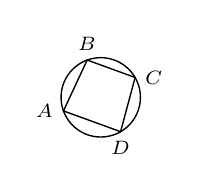
\begin{tikzpicture}[scale=0.42]
\draw (0,0) circle (1.2);
\draw (200:1.2) coordinate (A)--(110:1.2) coordinate (B)--(30:1.2) coordinate (C)--(-60:1.2) coordinate (D)--cycle;
\node[left,lb] at (A){$A$}; \node[above,lb] at (B){$B$}; \node[right,lb] at (C){$C$}; \node[below,lb] at (D){$D$};
\end{tikzpicture}\quad
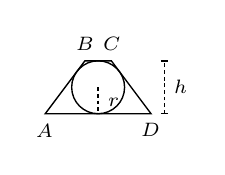
\begin{tikzpicture}[scale=0.42]
\coordinate (A) at (0,0); \coordinate (D) at (3.2,0); \coordinate (C) at (2.0,1.6); \coordinate (B) at (1.2,1.6);
\draw (A)--(B)--(C)--(D)--cycle; \draw (1.6,0.8) circle (0.8);
\draw[hid] (1.6,0.8)--(1.6,0); \node[right,lb] at (1.6,0.35) {$r$};
\draw[hid] (3.6,0)--(3.6,1.6); \draw (3.5,0)--(3.7,0) (3.5,1.6)--(3.7,1.6); \node[right,lb] at (3.6,0.8) {$h$};
\node[below,lb] at (A){$A$}; \node[above,lb] at (B){$B$}; \node[above,lb] at (C){$C$}; \node[below,lb] at (D){$D$};
\end{tikzpicture}}
\begin{fbx}
Вписанный: $\angle A+\angle C=\angle B+\angle D=180^\circ$\\
Описанный: $AB+CD=BC+AD$\\
Трапеция около окружности: $h=2r$
\end{fbx}

\newpage %24
\task{1}{Прототипы}
\proto{1.1}{Высота и медиана из прямого угла}
\fig{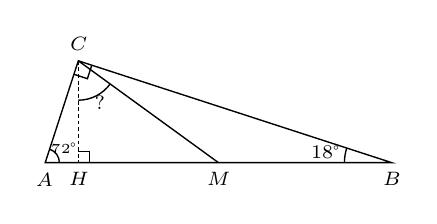
\begin{tikzpicture}[scale=1.0]
\coordinate (A) at (0,0); \coordinate (B) at (4.4,0); \coordinate (C) at (0.4202,1.2931);
\coordinate (H) at (0.4202,0); \coordinate (M) at (2.2,0);
\draw (A)--(B)--(C)--cycle; \draw (C)--(M); \draw[hid] (C)--(H);
\pic[draw,angle radius=1.8mm] {right angle=A--C--B};
\pic[draw,angle radius=1.4mm] {right angle=C--H--B};
\pic[draw,angle radius=1.8mm] {angle=B--A--C}; \node[lb] at ($(A)+(36:0.3)$) {\tiny$72^\circ$};
\pic[draw,angle radius=6mm] {angle=C--B--A}; \node[lb] at ($(B)+(171:0.85)$) {$18^\circ$};
\pic[draw,angle radius=5mm] {angle=H--C--M}; \node[lb] at ($(C)+(-63:0.6)$) {?};
\node[below,lb] at (A) {$A$}; \node[below,lb] at (B) {$B$}; \node[above,lb] at (C) {$C$};
\node[below,lb] at (H) {$H$}; \node[below,lb] at (M) {$M$};
\end{tikzpicture}}
\begin{ex}
Острые углы прямоугольного треугольника равны $72^\circ$ и~$18^\circ$. Найдите угол между высотой и~медианой, проведёнными из вершины прямого угла. Ответ дайте в~градусах.
\end{ex}
\sol $CM=AM\Rightarrow\angle ACM=\angle A=72^\circ$;\\
$\angle ACH=\angle B=18^\circ$ \ (с.~18).\\[0.5mm]
$\angle HCM=72^\circ-18^\circ=54^\circ$
\ans{54}
\begin{trap}
\warn Ответ~— \textbf{разность} острых углов, а не $90^\circ-72^\circ$.
\end{trap}

\newpage %25
\proto{1.2}{Угол между высотами}
\fig{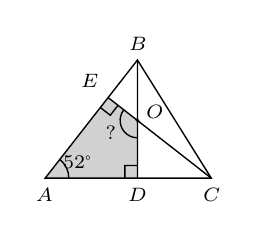
\begin{tikzpicture}[scale=0.62]
\coordinate (A) at (0,0); \coordinate (B) at (1.889,2.418); \coordinate (C) at (3.4,0);
\coordinate (D) at ($(A)!(B)!(C)$); \coordinate (E) at ($(A)!(C)!(B)$);
\coordinate (O) at (intersection of B--D and C--E);
\fill[black!18] (A)--(D)--(O)--(E)--cycle;
\draw (A)--(B)--(C)--cycle; \draw (B)--(D) (C)--(E);
\pic[draw,angle radius=1.6mm] {right angle=B--D--A};
\pic[draw,angle radius=1.6mm] {right angle=A--E--C};
\pic[draw,angle radius=3mm] {angle=D--A--E}; \node[lb] at ($(A)+(26:0.75)$) {$52^\circ$};
\pic[draw,angle radius=2.2mm] {angle=E--O--D}; \node[lb] at ($(O)+(205:0.6)$) {?};
\fill (O) circle (0.04);
\node[below,lb] at (A) {$A$}; \node[above,lb] at (B) {$B$}; \node[below,lb] at (C) {$C$};
\node[below,lb] at (D) {$D$}; \node[above left,lb] at (E) {$E$}; \node[lb] at ($(O)+(26:0.4)$) {$O$};
\end{tikzpicture}}
\begin{ex}
В треугольнике $ABC$ угол $A$ равен $52^\circ$, углы $B$ и~$C$~— острые, высоты $BD$ и~$CE$ пересекаются в~точке $O$. Найдите угол $DOE$. Ответ дайте в~градусах.
\end{ex}
\sol В четырёхугольнике $ADOE$ сумма углов $360^\circ$, $\angle D=\angle E=90^\circ$ \ (с.~14):\\[0.5mm]
$\angle DOE=360^\circ-90^\circ-90^\circ-52^\circ=128^\circ$
\ans{128}
\begin{trap}
\warn $\angle DOE$ тупой. Острый угол $52^\circ$~— это смежный с~ним $\angle BOE$.
\end{trap}

\newpage %26
\proto{1.3}{Высота к боковой стороне}
\fig{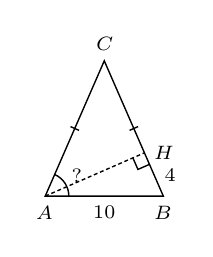
\begin{tikzpicture}[scale=0.6]
\coordinate (A) at (0,0); \coordinate (B) at (2.5,0); \coordinate (C) at (1.25,2.864);
\coordinate (H) at (2.1,0.9165);
\draw (A)--(B)--(C)--cycle; \draw[hid] (A)--(H);
\pic[draw,angle radius=1.6mm] {right angle=A--H--B};
\pic[draw,angle radius=3mm] {angle=B--A--C}; \node[lb] at ($(A)+(33:0.8)$) {?};
\draw ($(A)!0.5!(C)+(-0.09,0.04)$)--++(0.18,-0.08); \draw ($(B)!0.5!(C)+(-0.09,-0.04)$)--++(0.18,0.08);
\node[below,lb] at (1.25,0) {10}; \node[right,lb] at (2.32,0.45) {4};
\node[below,lb] at (A) {$A$}; \node[below,lb] at (B) {$B$}; \node[above,lb] at (C) {$C$}; \node[right,lb] at (H) {$H$};
\end{tikzpicture}}
\begin{ex}
В треугольнике $ABC$ $AC=BC$, $AB=10$, $AH$~— высота, $BH=4$. Найдите косинус угла $BAC$.
\end{ex}
\sol $AC=BC\Rightarrow\angle BAC=\angle ABC$ \ (с.~14).\\[0.5mm]
$\triangle ABH$: $\cos B=\dfrac{BH}{AB}=\dfrac4{10}=0{,}4$ \ (с.~18)
\ans{0,4}
\begin{trap}
\warn Угла $A$ в~треугольнике $ABH$ нет~— ищи равный ему угол $B$.
\end{trap}

\newpage %27
\proto{1.4}{Касательная и секущая через центр}
\fig{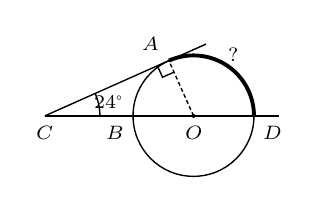
\begin{tikzpicture}[scale=0.64]
\coordinate (O) at (0,0); \coordinate (C) at (-2.95,0);
\coordinate (A) at (114:1.2); \coordinate (B) at (-1.2,0); \coordinate (D) at (1.2,0);
\draw (O) circle (1.2);
\draw[line width=1.4pt] (1.2,0) arc[start angle=0,end angle=114,radius=1.2];
\draw (C)--($(C)!1.3!(A)$); \draw (C)--(1.7,0); \draw[hid] (O)--(A);
\pic[draw,angle radius=1.6mm] {right angle=C--A--O};
\pic[draw,angle radius=7mm] {angle=O--C--A}; \node[lb] at ($(C)+(12:1.3)$) {$24^\circ$};
\fill (O) circle (0.04);
\node[below,lb] at (O) {$O$}; \node[below,lb] at (C) {$C$}; \node[above left,lb] at (A) {$A$};
\node[below left,lb] at (B) {$B$}; \node[below right,lb] at (D) {$D$};
\node[lb] at (57:1.45) {?};
\end{tikzpicture}}
\begin{ex}
Угол $ACO$ равен $24^\circ$. Его сторона $CA$ касается окружности с~центром $O$, сторона $CO$ пересекает окружность в~точках $B$ и~$D$. Найдите градусную меру дуги $AD$, заключённой внутри угла.
\end{ex}
\sol $OA\perp CA$ \ (с.~23): $\angle AOC=90^\circ-24^\circ=66^\circ$.\\[0.5mm]
$\angle AOD=180^\circ-66^\circ=114^\circ$ \ (с.~13);\ $\cup AD=114^\circ$ \ (с.~22)
\ans{114}
\begin{trap}
\warn $66^\circ$~— это дуга $AB$, а не $AD$.
\end{trap}

\newpage %28
\proto{1.5}{Прямоугольная трапеция около окружности}
\fig{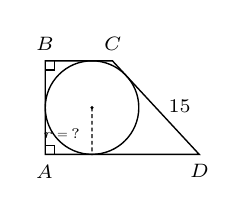
\begin{tikzpicture}[scale=0.72]
\coordinate (A) at (0,0); \coordinate (D) at (2.715,0); \coordinate (C) at (1.185,1.65); \coordinate (B) at (0,1.65);
\draw (A)--(B)--(C)--(D)--cycle;
\draw (A)++(0,0.16)--++(0.16,0)--++(0,-0.16); \draw (B)++(0,-0.16)--++(0.16,0)--++(0,0.16);
\coordinate (I) at (0.825,0.825); \draw (I) circle (0.825); \fill (I) circle (0.03);
\draw[hid] (I)--(0.825,0); \node[left,lb] at (0.8,0.36) {\tiny$r=?$};
\node[right,lb] at (2,0.85) {15};
\node[below,lb] at (A) {$A$}; \node[above,lb] at (B) {$B$}; \node[above,lb] at (C) {$C$}; \node[below,lb] at (D) {$D$};
\end{tikzpicture}}
\begin{ex}
Периметр прямоугольной трапеции, описанной около окружности, равен $52$, её большая боковая сторона равна $15$. Найдите радиус окружности.
\end{ex}
\sol $AB+CD=BC+AD=52:2=26$ \ (с.~23).\\[0.5mm]
$AB=26-15=11$. $AB\perp AD$, поэтому $AB=h=2r$:\ $r=5{,}5$
\ans{5,5}
\begin{trap}
\warn Меньшая боковая сторона равна \textbf{диаметру}, а не радиусу.
\end{trap}

\newpage %29
\proto{1.6}{Тупой угол и описанная окружность}
\fig{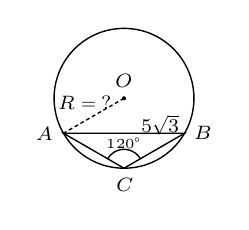
\begin{tikzpicture}[scale=0.74]
\coordinate (O) at (0,0);
\coordinate (A) at (210:1.2); \coordinate (B) at (330:1.2); \coordinate (C) at (270:1.2);
\draw (O) circle (1.2); \draw (A)--(B)--(C)--cycle;
\draw[hid] (O)--(A); \node[lb] at (-0.66,-0.08) {$R=?$};
\pic[draw,angle radius=2.4mm] {angle=B--C--A}; \node[lb] at ($(C)+(90:0.42)$) {\tiny$120^\circ$};
\fill (O) circle (0.035);
\node[above,lb] at (O) {$O$}; \node[left,lb] at (A) {$A$}; \node[right,lb] at (B) {$B$}; \node[below,lb] at (C) {$C$};
\node[lb] at (0.62,-0.46) {$5\sqrt3$};
\end{tikzpicture}}
\begin{ex}
В треугольнике $ABC$ сторона $AB$ равна $5\sqrt3$, угол $C$ равен $120^\circ$. Найдите радиус описанной около этого треугольника окружности.
\end{ex}
\sol По теореме синусов \ (с.~17):\\[0.5mm]
$2R=\dfrac{AB}{\sin120^\circ}=\dfrac{5\sqrt3}{\sqrt3/2}=10$,\quad $R=5$
\ans{5}
\begin{trap}
\warn $\sin120^\circ=\sin60^\circ=\dfrac{\sqrt3}{2}$~— синус тупого угла положителен.
\end{trap}

%==================== ЗАДАНИЕ 2 ====================
\newpage %30
\task{2}{Векторы}
\tpage{2}{Векторы}
\blk{Что спрашивают}
Длину вектора, скалярное произведение или косинус угла. Векторы даны координатами, длинами и~углом или рисунком на клетках.
\blk{Алгоритм}
\begin{enumerate}
\item Найди координаты каждого вектора: на клетках~— методом треугольника (с.~31), по точкам~— конец минус начало (с.~32).
\item Действия выполняй покоординатно.
\item Длина, скалярное произведение, косинус~— по формулам (с.~31, 33).
\item Проверь знаки: влево и~вниз~— «$-$».
\end{enumerate}
\blk{В бланк}
Скалярное произведение~— \textbf{число}, может быть отрицательным. Косинус~— от $-1$ до~$1$.

\newpage %31
\blk{Координаты через треугольник}
\fig{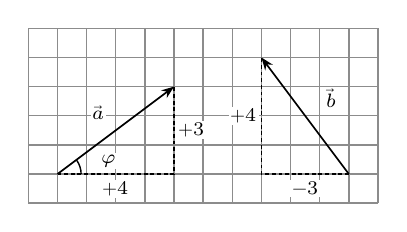
\begin{tikzpicture}[scale=0.37]
\draw[black!45,line width=0.5pt] (0,0) grid (12,6);
\coordinate (S) at (1,1); \coordinate (E) at (5,1); \coordinate (T) at (5,4);
\draw[hid,line width=0.6pt] (1,1)--(5,1)--(5,4);
\draw[hid,line width=0.6pt] (11,1)--(8,1)--(8,5);
\draw[vec] (1,1)--(5,4); \draw[vec] (11,1)--(8,5);
\pic[draw,angle radius=3mm] {angle=E--S--T};
\node[lb,fill=white,inner sep=0.6pt] at (3,0.5) {$+4$}; \node[lb,fill=white,inner sep=0.6pt] at (5.6,2.5) {$+3$};
\node[lb,fill=white,inner sep=0.6pt] at (9.5,0.5) {$-3$}; \node[lb,fill=white,inner sep=0.6pt] at (7.4,3) {$+4$};
\node[lb,fill=white,inner sep=0.6pt] at (2.4,3.1) {$\vec a$}; \node[lb,fill=white,inner sep=0.6pt] at (10.4,3.6) {$\vec b$};
\node[lb,fill=white,inner sep=0.6pt] at (2.75,1.45) {$\varphi$};
\end{tikzpicture}}
\begin{fbx}
Вектор~— гипотенуза. От начала~— горизонтальный катет: это $x$; от него к~концу~— вертикальный: это $y$.
\end{fbx}
\begin{fbx}
Вправо, вверх~— «$+$»; влево, вниз~— «$-$». На клетках длины катетов считаем по клеточкам.
\end{fbx}
\begin{fbx}
$|\vec a|=\sqrt{x^2+y^2}$\qquad $x=|\vec a|\cos\varphi$,\ \ $y=|\vec a|\sin\varphi$\\[0.3mm]
($\varphi$~— угол поворота от оси $Ox$ к~вектору)
\end{fbx}
На рисунке: $\vec a(4;\,3)$,\ $\vec b(-3;\,4)$,\ $|\vec a|=|\vec b|=5$.

\newpage %32
\blk{Координаты и действия}
\fig{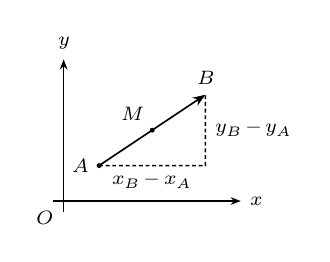
\begin{tikzpicture}[scale=0.45]
\axes{-0.3}{5}{-0.3}{4}
\coordinate (A) at (1,1); \coordinate (B) at (4,3); \coordinate (M) at (2.5,2);
\draw[vec] (A)--(B);
\fill (A) circle (0.07); \fill (M) circle (0.07);
\node[left,lb] at (A) {$A$}; \node[above,lb] at (B) {$B$}; \node[above left,lb] at (M) {$M$};
\draw[hid] (A)--(4,1)--(B);
\node[below,lb] at (2.5,1) {$x_B-x_A$}; \node[right,lb] at (4,2) {$y_B-y_A$};
\end{tikzpicture}\quad
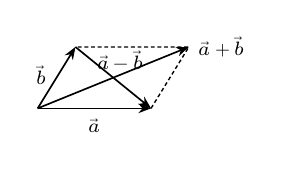
\begin{tikzpicture}[scale=0.6]
\coordinate (O) at (0,0); \coordinate (A) at (2.4,0); \coordinate (B) at (0.8,1.3); \coordinate (S) at (3.2,1.3);
\draw[hid] (A)--(S)--(B);
\draw[vec] (O)--(A); \node[below,lb] at (1.2,0) {$\vec a$};
\draw[vec] (O)--(B); \node[left,lb] at (0.4,0.7) {$\vec b$};
\draw[vec] (O)--(S); \node[right,lb] at (S) {$\vec a+\vec b$};
\draw[vec] (B)--(A); \node[lb] at (1.75,1.02) {$\vec a-\vec b$};
\end{tikzpicture}}
\begin{fbx}
$\overrightarrow{AB}=(x_B-x_A;\ y_B-y_A)$~— конец минус начало
\end{fbx}
\begin{fbx}
$\vec a(x_1;\,y_1)$, $\vec b(x_2;\,y_2)$:\\[0.3mm]
$\vec a\pm\vec b=(x_1\pm x_2;\ y_1\pm y_2)$\qquad $k\vec a=(kx_1;\ ky_1)$
\end{fbx}
\begin{fbx}
Середина $M$ отрезка $AB$: $\Bigl(\dfrac{x_A+x_B}{2};\ \dfrac{y_A+y_B}{2}\Bigr)$
\end{fbx}
\begin{fbx}
$\vec a\parallel\vec b$:\ координаты пропорциональны, $\dfrac{x_1}{x_2}=\dfrac{y_1}{y_2}$
\end{fbx}

\newpage %33
\blk{Скалярное произведение}
\fig{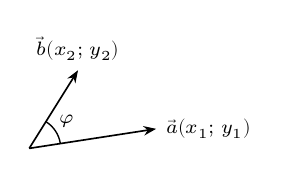
\begin{tikzpicture}[scale=0.62]
\coordinate (O) at (0,0); \coordinate (A) at (2.6,0.4); \coordinate (B) at (1,1.6);
\draw[vec] (O)--(A) node[right,lb]{$\vec a(x_1;\,y_1)$}; \draw[vec] (O)--(B) node[above,lb]{$\vec b(x_2;\,y_2)$};
\pic[draw,angle radius=4mm] {angle=A--O--B}; \node[lb] at ($(O)+(35:0.95)$) {$\varphi$};
\end{tikzpicture}}
\begin{fbx}
$\vec a\cdot\vec b=|\vec a|\,|\vec b|\cos\varphi=x_1x_2+y_1y_2$
\end{fbx}
\begin{fbx}
$\cos\varphi=\dfrac{x_1x_2+y_1y_2}{|\vec a|\,|\vec b|}$
\end{fbx}
\begin{fbx}
$\vec a\perp\vec b\ \Leftrightarrow\ \vec a\cdot\vec b=0$\qquad $\vec a\cdot\vec a=|\vec a|^2$\\[0.5mm]
$|\vec a\pm\vec b|^2=|\vec a|^2\pm2\,\vec a\cdot\vec b+|\vec b|^2$
\end{fbx}
Угол $\varphi$ измеряют между векторами, отложенными от одной точки. $\varphi$ острый~— $\vec a\cdot\vec b>0$, тупой~— $\vec a\cdot\vec b<0$.

\newpage %34
\task{2}{Прототипы}
\proto{2.1}{Три вектора на клетках, дробные коэффициенты}
\fig{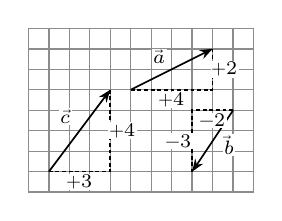
\begin{tikzpicture}[scale=0.26]
\draw[black!45,line width=0.5pt] (0,0) grid (11,8);
\draw[hid,line width=0.6pt] (5,5)--(9,5)--(9,7);
\draw[hid,line width=0.6pt] (10,4)--(8,4)--(8,1);
\draw[hid,line width=0.6pt] (1,1)--(4,1)--(4,5);
\draw[vec] (5,5)--(9,7); \draw[vec] (10,4)--(8,1); \draw[vec] (1,1)--(4,5);
\node[lb,fill=white,inner sep=0.5pt] at (6.4,6.6) {$\vec a$};
\node[lb,fill=white,inner sep=0.5pt] at (9.8,2.3) {$\vec b$};
\node[lb,fill=white,inner sep=0.5pt] at (1.8,3.7) {$\vec c$};
\node[lb,fill=white,inner sep=0.4pt] at (7,4.5) {$+4$}; \node[lb,fill=white,inner sep=0.4pt] at (9.6,6) {$+2$};
\node[lb,fill=white,inner sep=0.4pt] at (9,3.5) {$-2$}; \node[lb,fill=white,inner sep=0.4pt] at (7.35,2.5) {$-3$};
\node[lb,fill=white,inner sep=0.4pt] at (2.5,0.5) {$+3$}; \node[lb,fill=white,inner sep=0.4pt] at (4.6,3) {$+4$};
\end{tikzpicture}}
\begin{ex}
Векторы на рисунке имеют целые координаты. Найдите длину вектора $0{,}5\vec a+1{,}5\vec b-\vec c$.
\end{ex}
\sol По клеткам (с.~31): $\vec a(4;2)$, $\vec b(-2;-3)$, $\vec c(3;4)$.\\[0.5mm]
$(2-3-3;\ 1-4{,}5-4)=(-4;\,-7{,}5)$ \ (с.~32)\\[0.5mm]
$\sqrt{16+56{,}25}=\sqrt{72{,}25}=8{,}5$
\ans{8,5}
\begin{trap}
\warn У $\vec b$ катеты идут влево и~вниз: обе координаты $<0$.
\end{trap}

\newpage %35
\proto{2.2}{Векторы не из начала координат}
\fig{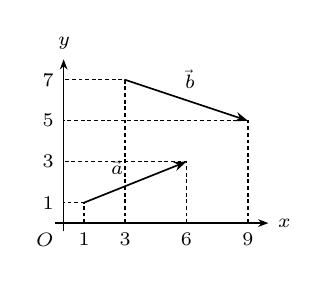
\begin{tikzpicture}[scale=0.26]
\axes{-0.4}{10}{-0.4}{8}
\draw[hid] (1,0)--(1,1)--(0,1) (6,0)--(6,3)--(0,3) (3,0)--(3,7)--(0,7) (9,0)--(9,5)--(0,5);
\draw[vec] (1,1)--(6,3); \draw[vec] (3,7)--(9,5);
\node[above left,lb] at (3.4,1.9) {$\vec a$}; \node[above,lb] at (6.2,6.1) {$\vec b$};
\foreach \x in {1,3,6,9} \node[below,lb] at (\x,0) {\x};
\foreach \y in {1,3,5,7} \node[left,lb] at (0,\y) {\y};
\end{tikzpicture}}
\begin{ex}
Векторы $\vec a$ и~$\vec b$ изображены на рисунке. Найдите скалярное произведение $\vec a\cdot\vec b$.
\end{ex}
\sol Конец минус начало \ (с.~32):\\[0.5mm]
$\vec a(6-1;\ 3-1)=(5;\,2)$,\ $\vec b(9-3;\ 5-7)=(6;\,-2)$\\[0.5mm]
$\vec a\cdot\vec b=5\cdot6+2\cdot(-2)=26$ \ (с.~33)
\ans{26}
\begin{trap}
\warn Не координаты конца: $6\cdot9+3\cdot5=69$~— ошибка.
\end{trap}

\newpage %36
\proto{2.3}{Скалярное произведение разности}
\fig{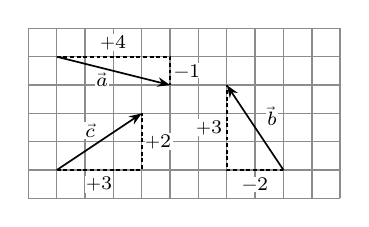
\begin{tikzpicture}[scale=0.36]
\draw[black!45,line width=0.5pt] (0,0) grid (11,6);
\draw[hid,line width=0.6pt] (1,5)--(5,5)--(5,4);
\draw[hid,line width=0.6pt] (9,1)--(7,1)--(7,4);
\draw[hid,line width=0.6pt] (1,1)--(4,1)--(4,3);
\draw[vec] (1,5)--(5,4); \draw[vec] (9,1)--(7,4); \draw[vec] (1,1)--(4,3);
\node[lb,fill=white,inner sep=0.5pt] at (2.6,4.2) {$\vec a$};
\node[lb,fill=white,inner sep=0.5pt] at (8.6,2.9) {$\vec b$};
\node[lb,fill=white,inner sep=0.5pt] at (2.2,2.4) {$\vec c$};
\node[lb,fill=white,inner sep=0.4pt] at (3,5.5) {$+4$}; \node[lb,fill=white,inner sep=0.4pt] at (5.6,4.5) {$-1$};
\node[lb,fill=white,inner sep=0.4pt] at (8,0.5) {$-2$}; \node[lb,fill=white,inner sep=0.4pt] at (6.4,2.5) {$+3$};
\node[lb,fill=white,inner sep=0.4pt] at (2.5,0.5) {$+3$}; \node[lb,fill=white,inner sep=0.4pt] at (4.6,2) {$+2$};
\end{tikzpicture}}
\begin{ex}
Векторы $\vec a$, $\vec b$, $\vec c$ на рисунке имеют целые координаты. Найдите $(\vec a-\vec b)\cdot\vec c$.
\end{ex}
\sol По клеткам \ (с.~31): $\vec a(4;\,-1)$, $\vec b(-2;\,3)$, $\vec c(3;\,2)$.\\[0.5mm]
$\vec a-\vec b=(4+2;\ -1-3)=(6;\,-4)$ \ (с.~32)\\[0.5mm]
$(\vec a-\vec b)\cdot\vec c=18-8=10$ \ (с.~33)
\ans{10}
\begin{trap}
\warn Вычитая отрицательную координату, меняй знак: $4-(-2)=6$.
\end{trap}

\newpage %37
\proto{2.4}{Косинус угла по рисунку}
\fig{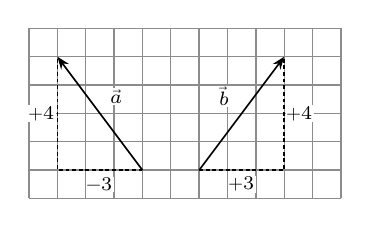
\begin{tikzpicture}[scale=0.36]
\draw[black!45,line width=0.5pt] (0,0) grid (11,6);
\draw[hid,line width=0.6pt] (4,1)--(1,1)--(1,5);
\draw[hid,line width=0.6pt] (6,1)--(9,1)--(9,5);
\draw[vec] (4,1)--(1,5); \draw[vec] (6,1)--(9,5);
\node[lb,fill=white,inner sep=0.5pt] at (3.1,3.6) {$\vec a$};
\node[lb,fill=white,inner sep=0.5pt] at (6.9,3.6) {$\vec b$};
\node[lb,fill=white,inner sep=0.4pt] at (2.5,0.5) {$-3$}; \node[lb,fill=white,inner sep=0.4pt] at (0.45,3) {$+4$};
\node[lb,fill=white,inner sep=0.4pt] at (7.5,0.5) {$+3$}; \node[lb,fill=white,inner sep=0.4pt] at (9.55,3) {$+4$};
\end{tikzpicture}}
\begin{ex}
Векторы $\vec a$ и~$\vec b$ на рисунке имеют целые координаты. Найдите косинус угла между ними.
\end{ex}
\sol Треугольники \ (с.~31): $\vec a(-3;\,4)$, $|\vec a|=5$;\ $\vec b(3;\,4)$, $|\vec b|=5$.\\[0.5mm]
$\cos\varphi=\dfrac{-9+16}{5\cdot5}=\dfrac{7}{25}=0{,}28$ \ (с.~33)
\ans{0,28}
\begin{trap}
\warn Общего начала нет~— угол всё равно считают по координатам.
\end{trap}

%==================== ЗАДАНИЕ 3 ====================
\newpage %38
\task{3}{Стереометрия}
\tpage{3}{Стереометрия}
\blk{Что спрашивают}
Объём, площадь поверхности или длину. Часто: часть тела или «во сколько раз изменится».
\blk{Алгоритм}
\begin{enumerate}
\item Назови тело, выпиши формулу.
\item Часть тела~— сравни основание и~высоту части с~целым (с.~40–41).
\item «Во сколько раз», сечение $\parallel$ основанию~— найди $k$, возведи в~степень (с.~44).
\item Недостающий размер~— из прямоугольного треугольника.
\item Проверь, что просили: $V$, $S$, остаток или $V/\pi$.
\end{enumerate}
\blk{В бланк}
Просят $V/\pi$~— раздели на $\pi$. Число $\pi$ в~ответ не подставляем.

\newpage %39
\blk{Призма}
\fig{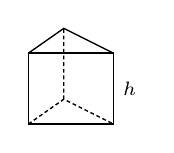
\begin{tikzpicture}[scale=0.45]
\draw (0,0)--(2.4,0)--(2.4,2)--(0,2)--cycle; \draw (0,2)--(1,2.7)--(2.4,2);
\draw[hid] (0,0)--(1,0.7)--(2.4,0) (1,0.7)--(1,2.7);
\node[right,lb] at (2.4,1) {$h$};
\end{tikzpicture}\quad
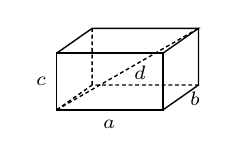
\begin{tikzpicture}[scale=0.45]
\draw (0,0) rectangle (3,1.6);
\draw (0,1.6)--(1,2.3)--(4,2.3)--(3,1.6);
\draw (4,2.3)--(4,0.7)--(3,0);
\draw[hid] (0,0)--(1,0.7)--(4,0.7) (1,0.7)--(1,2.3);
\draw[hid] (0,0)--(4,2.3);
\node[below,lb] at (1.5,0) {$a$}; \node[right,lb] at (3.5,0.3) {$b$};
\node[left,lb] at (0,0.8) {$c$}; \node[lb] at (2.35,1.05) {$d$};
\end{tikzpicture}}
\begin{fbx}
$V=S_{\text{осн}}\cdot h$\qquad Прямая: $S_{\text{бок}}=P_{\text{осн}}\cdot h$
\end{fbx}
\blk{Прямоугольный параллелепипед}
\begin{fbx}
$V=abc$\quad $d^2=a^2+b^2+c^2$\quad $S=2(ab+bc+ac)$
\end{fbx}
\begin{fbx}
Куб ($a=b=c$): $V=a^3$,\ $S=6a^2$,\ $d=a\sqrt3$
\end{fbx}

\newpage %40
\blk{Части многогранника}
\fig{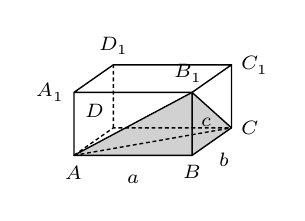
\begin{tikzpicture}[scale=0.5]
\coordinate (A) at (0,0); \coordinate (B) at (3,0); \coordinate (C) at (4,0.7); \coordinate (D) at (1,0.7);
\coordinate (A1) at (0,1.6); \coordinate (B1) at (3,1.6); \coordinate (C1) at (4,2.3); \coordinate (D1) at (1,2.3);
\fill[black!18] (A)--(B)--(C)--(B1)--cycle;
\draw (A)--(B)--(C)--(C1)--(D1)--(A1)--cycle (A1)--(B1)--(C1) (B)--(B1);
\draw[hid] (A)--(D)--(C) (D)--(D1);
\draw (A)--(B1)--(C); \draw[hid] (A)--(C);
\node[below,lb] at (A) {$A$}; \node[below,lb] at (B) {$B$}; \node[right,lb] at (C) {$C$}; \node[above left,lb] at (D) {$D$};
\node[left,lb] at (A1) {$A_1$}; \node[above,lb] at ($(B1)+(-0.1,0)$) {$B_1$}; \node[right,lb] at (C1) {$C_1$}; \node[above,lb] at (D1) {$D_1$};
\node[below,lb] at (1.5,-0.25) {$a$}; \node[below right,lb] at (3.45,0.3) {$b$}; \node[right,lb] at (3,0.85) {$c$};
\end{tikzpicture}}
\begin{fbx}
$V_{ABCB_1}=\tfrac13\cdot\tfrac{ab}{2}\cdot c=\dfrac{abc}{6}$\qquad $V_{ABCDB_1}=\dfrac{abc}{3}$
\end{fbx}
\fig{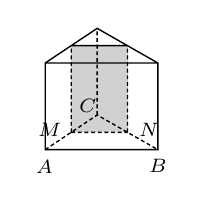
\begin{tikzpicture}[scale=0.55]
\coordinate (A) at (0,0); \coordinate (B) at (2.6,0); \coordinate (C) at (1.2,0.8);
\coordinate (A1) at (0,2); \coordinate (B1) at (2.6,2); \coordinate (C1) at (1.2,2.8);
\coordinate (M) at (0.6,0.4); \coordinate (N) at (1.9,0.4); \coordinate (M1) at (0.6,2.4); \coordinate (N1) at (1.9,2.4);
\fill[black!18] (M)--(N)--(N1)--(M1)--cycle;
\draw (A)--(B)--(B1)--(A1)--cycle (A1)--(C1)--(B1) (M1)--(N1);
\draw[hid] (A)--(C)--(B) (C)--(C1) (M)--(N) (M)--(M1) (N)--(N1);
\node[below,lb] at (A) {$A$}; \node[below,lb] at (B) {$B$}; \node[lb] at (0.98,1.0) {$C$};
\node[left,lb] at ($(M)+(-0.05,0.05)$) {$M$}; \node[right,lb] at ($(N)+(0.05,0.05)$) {$N$};
\end{tikzpicture}}
\begin{fbx}
Плоскость через среднюю линию $MN\parallel$ боковому ребру. Отсечённая призма: $S_{\text{осн}}$ и~$V$ $\times\tfrac14$,\ $S_{\text{бок}}$ $\times\tfrac12$
\end{fbx}

\newpage %41
\blk{Пирамида}
\fig{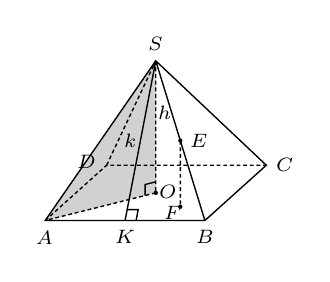
\begin{tikzpicture}[scale=0.78]
\coordinate (A) at (0,0); \coordinate (B) at (2.6,0); \coordinate (C) at (3.6,0.9); \coordinate (D) at (1,0.9);
\coordinate (O) at (1.8,0.45); \coordinate (S) at (1.8,2.6); \coordinate (K) at (1.3,0);
\coordinate (E) at (2.2,1.3); \coordinate (F) at (2.2,0.225);
\fill[black!18] (S)--(O)--(A)--cycle;
\draw (A)--(B)--(C)--(S)--cycle (S)--(B) (S)--(K);
\draw[hid] (A)--(D)--(C) (D)--(S) (S)--(O) (O)--(A) (E)--(F);
\pic[draw,angle radius=1.4mm] {right angle=S--K--B};
\pic[draw,angle radius=1.4mm] {right angle=S--O--A};
\fill (O) circle (0.035); \fill (E) circle (0.035); \fill (F) circle (0.035);
\node[above,lb] at (S) {$S$}; \node[below,lb] at (A) {$A$}; \node[below,lb] at (B) {$B$};
\node[right,lb] at (C) {$C$}; \node[left,lb] at ($(D)+(-0.02,0.05)$) {$D$}; \node[below,lb] at (K) {$K$};
\node[lb] at (1.99,0.47) {$O$}; \node[right,lb] at (E) {$E$}; \node[lb] at (2.05,0.12) {$F$};
\node[lb] at (1.95,1.75) {$h$}; \node[lb] at (1.38,1.3) {$k$};
\end{tikzpicture}}
\begin{fbx}
$V=\tfrac13\,S_{\text{осн}}\cdot h$\qquad $S_{\text{бок}}=\tfrac12\,P_{\text{осн}}\cdot k$
\end{fbx}
\textbf{Правильная:} в основании правильный многоугольник, $SO$~— в~его центр $O$, $k=SK$~— апофема.
\begin{fbx}
$\triangle SOA$, $\triangle SOK$~— прямоугольные: $SA^2=h^2+OA^2$
\end{fbx}
\begin{fbx}
$E$~— середина $SB$: высота $EF=\tfrac h2$\\
Общие основание и~высота с~призмой: $V_{\text{пир}}=\tfrac13\,V_{\text{пр}}$
\end{fbx}

\newpage %42
\fig{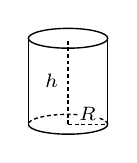
\begin{tikzpicture}[scale=0.42]
\cyl{0}{1.2}{2.6}{0}
\draw[hid] (0,0)--(0,2.6) (0,0)--(1.2,0);
\node[left,lb] at (0,1.3) {$h$}; \node[above,lb,fill=white,inner sep=0.4pt] at (0.6,0.05) {$R$};
\end{tikzpicture}\qquad
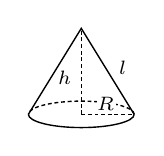
\begin{tikzpicture}[scale=0.42]
\cone{1.6}{2.6}
\draw[hid] (0,0)--(0,2.6) (0,0)--(1.6,0);
\node[left,lb] at (0,1.1) {$h$}; \node[above,lb,fill=white,inner sep=0.4pt] at (0.75,0.05) {$R$}; \node[right,lb] at (0.85,1.4) {$l$};
\end{tikzpicture}}
\blk{Цилиндр}
\begin{fbx}
$V=\pi R^2h$\quad $S_{\text{бок}}=2\pi Rh$\quad $S_{\text{полн}}=2\pi R(R+h)$
\end{fbx}
\blk{Конус}
\begin{fbx}
$V=\tfrac13\pi R^2h$\quad $l^2=R^2+h^2$\\[0.4mm]
$S_{\text{бок}}=\pi Rl$\quad $S_{\text{полн}}=\pi R(R+l)$
\end{fbx}
\begin{fbx}
Осевое сечение: цилиндра~— прямоугольник $2R\times h$, конуса~— равнобедренный треугольник с~основанием $2R$ и~высотой $h$
\end{fbx}

\newpage %43
\blk{Шар}
\fig{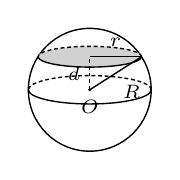
\begin{tikzpicture}[scale=0.6]
\draw (0,0) circle (1.3);
\draw (-1.3,0) arc[start angle=180,end angle=360,x radius=1.3,y radius=0.3];
\draw[hid] (1.3,0) arc[start angle=0,end angle=180,x radius=1.3,y radius=0.3];
\fill[black!18] (0,0.7) ellipse[x radius=1.095,y radius=0.22];
\draw (-1.095,0.7) arc[start angle=180,end angle=360,x radius=1.095,y radius=0.22];
\draw[hid] (1.095,0.7) arc[start angle=0,end angle=180,x radius=1.095,y radius=0.22];
\fill (0,0) circle (0.035); \node[below,lb] at (0,0) {$O$};
\draw[hid] (0,0)--(0,0.7); \node[left,lb] at (0,0.33) {$d$};
\draw (0,0.7)--(1.095,0.7); \node[above,lb] at (0.55,0.7) {$r$};
\draw (0,0)--(1.095,0.7); \node[below right,lb] at (0.5,0.3) {$R$};
\end{tikzpicture}}
\begin{fbx}
$V=\tfrac43\,\pi R^3$\qquad $S=4\pi R^2$
\end{fbx}
\blk{Сечение шара}
Сечение шара плоскостью~— круг.
\begin{fbx}
$r^2=R^2-d^2$, $d$~— расстояние от центра $O$ до плоскости\\[0.4mm]
Площадь сечения: $\pi r^2$
\end{fbx}

\newpage %44
\blk{«Во сколько раз»}
\fig{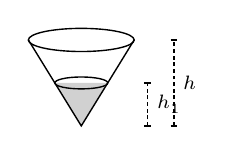
\begin{tikzpicture}[scale=0.42]
\fill[black!18] (0,0)--(-0.8,1.3)--(0.8,1.3)--cycle;
\draw (-1.6,2.6)--(0,0)--(1.6,2.6); \draw (0,2.6) ellipse[x radius=1.6,y radius=0.35];
\draw (0,1.3) ellipse[x radius=0.8,y radius=0.18];
\draw[hid] (2,0)--(2,1.3); \draw (1.9,0)--(2.1,0) (1.9,1.3)--(2.1,1.3); \node[right,lb] at (2,0.65) {$h_1$};
\draw[hid] (2.8,0)--(2.8,2.6); \draw (2.7,0)--(2.9,0) (2.7,2.6)--(2.9,2.6); \node[right,lb] at (2.8,1.3) {$h$};
\end{tikzpicture}\qquad
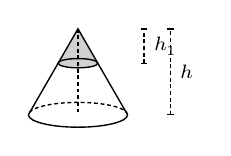
\begin{tikzpicture}[scale=0.42]
\fill[black!18] (0,2.6)--(-0.6,1.56) arc[start angle=180,end angle=360,x radius=0.6,y radius=0.14]--cycle;
\cone{1.5}{2.6}
\draw (0,1.56) ellipse[x radius=0.6,y radius=0.14];
\draw[hid] (0,2.6)--(0,0);
\draw (1.9,1.56)--(2.1,1.56) (1.9,2.6)--(2.1,2.6); \draw[hid] (2,1.56)--(2,2.6); \node[right,lb] at (2,2.08) {$h_1$};
\draw (2.7,0)--(2.9,0) (2.7,2.6)--(2.9,2.6); \draw[hid] (2.8,0)--(2.8,2.6); \node[right,lb] at (2.8,1.3) {$h$};
\end{tikzpicture}}
\begin{fbx}
Подобные тела, $k=\dfrac{h_1}{h}$: длины $\times k$, площади $\times k^2$, объёмы $\times k^3$
\end{fbx}
\begin{fbx}
Сечение конуса $\parallel$ основанию отсекает подобный конус; $h_1$ считают от вершины
\end{fbx}
\begin{itemize}
\item Сосуд-конус: $V_{\text{сосуда}}=V_{\text{жидк}}:k^3$, долить $V_{\text{сосуда}}-V_{\text{жидк}}$.
\item Радиус цилиндра $\times2$~— объём $\times4$.
\item Жидкость перелили~— объём тот же.
\end{itemize}

\newpage %45
\blk{Комбинации тел}
\fig{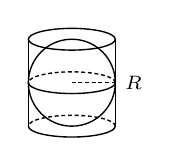
\begin{tikzpicture}[scale=0.46]
\cyl{0}{1.2}{2.4}{0}
\begin{scope}[shift={(0,1.2)}]\ball{1.2}\end{scope}
\draw[hid] (0,1.2)--(1.2,1.2); \node[right,lb] at (1.2,1.2) {$R$};
\end{tikzpicture}\quad
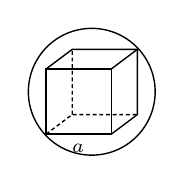
\begin{tikzpicture}[scale=0.46]
\cube{0}{0}{1.8}
\draw (1.26,1.17) circle (1.75);
\node[below,lb] at (0.9,0) {$a$};
\end{tikzpicture}\quad
\begin{tikzpicture}[scale=0.46]
\draw (0,0) circle (1.4);
\draw (-1.4,0) arc[start angle=180,end angle=360,x radius=1.4,y radius=0.32];
\draw[hid] (1.4,0) arc[start angle=0,end angle=180,x radius=1.4,y radius=0.32];
\draw (-1.4,0)--(0,1.4)--(1.4,0); \draw[hid] (0,0)--(0,1.4) (0,0)--(-1.4,0);
\fill (0,0) circle (0.07); \node[below,lb] at (0,-0.3) {$O$};
\node[right,lb] at (0.72,0.75) {$l$}; \node[lb] at (-0.75,0.3) {$R$};
\end{tikzpicture}}
\begin{fbx}
Шар в цилиндре: $h=2R$,\ $r_{\text{цил}}=R$\\
Куб в шаре: $a\sqrt3=2R$;\ шар в кубе: $a=2R$
\end{fbx}
\begin{fbx}
Конус в шаре, $O$~— центр основания:\\ $h=r=R$,\ $l=R\sqrt2$
\end{fbx}
\begin{fbx}
Общие основание и высота: $V_{\text{кон}}=\tfrac13\,V_{\text{цил}}$
\end{fbx}

\newpage %46
\task{3}{Прототипы}
\proto{3.1}{Пирамида внутри параллелепипеда}
\fig{\begin{tikzpicture}[scale=0.5]
\coordinate (A) at (0,0); \coordinate (B) at (3,0); \coordinate (C) at (4,0.7); \coordinate (D) at (1,0.7);
\coordinate (A1) at (0,1.6); \coordinate (B1) at (3,1.6); \coordinate (C1) at (4,2.3); \coordinate (D1) at (1,2.3);
\fill[black!18] (A)--(B)--(C)--(B1)--cycle;
\draw (A)--(B)--(C)--(C1)--(D1)--(A1)--cycle (A1)--(B1)--(C1) (B)--(B1);
\draw[hid] (A)--(D)--(C) (D)--(D1);
\draw (A)--(B1)--(C); \draw[hid] (A)--(C);
\node[below,lb] at (A) {$A$}; \node[below,lb] at (B) {$B$}; \node[right,lb] at (C) {$C$}; \node[above left,lb] at (D) {$D$};
\node[left,lb] at (A1) {$A_1$}; \node[above,lb] at ($(B1)+(-0.1,0)$) {$B_1$}; \node[right,lb] at (C1) {$C_1$}; \node[above,lb] at (D1) {$D_1$};
\node[below,lb] at (1.5,-0.25) {8}; \node[below right,lb] at (3.45,0.3) {6}; \node[lb] at (2.8,0.9) {5};
\node[lb] at (1.9,0.64) {?};
\end{tikzpicture}}
\begin{ex}
В прямоугольном параллелепипеде $ABCDA_1B_1C_1D_1$ $AB=8$, $BC=6$, $BB_1=5$. Найдите объём многогранника с~вершинами $A$, $B$, $C$, $B_1$.
\end{ex}
\sol Это пирамида: основание $ABC$, высота $BB_1$ \ (с.~40).\\[0.5mm]
$V=\tfrac13\cdot\tfrac{8\cdot6}{2}\cdot5=40$
\ans{40}
\begin{trap}
\warn Основание~— половина прямоугольника: $V=\dfrac{abc}{6}$, а не $\dfrac{abc}{3}$.
\end{trap}

\newpage %47
\proto{3.2}{Призма, отсечённая через среднюю линию}
\fig{\begin{tikzpicture}[scale=0.46]
\coordinate (A) at (0,0); \coordinate (B) at (2.6,0); \coordinate (C) at (1.2,0.8);
\coordinate (A1) at (0,2); \coordinate (B1) at (2.6,2); \coordinate (C1) at (1.2,2.8);
\coordinate (M) at (0.6,0.4); \coordinate (N) at (1.9,0.4); \coordinate (M1) at (0.6,2.4); \coordinate (N1) at (1.9,2.4);
\fill[black!18] (M)--(N)--(N1)--(M1)--cycle;
\draw (A)--(B)--(B1)--(A1)--cycle (A1)--(C1)--(B1) (M1)--(N1);
\draw[hid] (A)--(C)--(B) (C)--(C1) (M)--(N) (M)--(M1) (N)--(N1);
\node[below,lb] at (A) {$A$}; \node[below,lb] at (B) {$B$}; \node[lb] at (0.98,1.0) {$C$};
\node[left,lb] at ($(M)+(-0.05,0.05)$) {$M$}; \node[right,lb] at ($(N)+(0.05,0.05)$) {$N$};
\node[right,lb] at (2.7,1.2) {$S_{\text{бок}}=46$}; \node[lb] at (1.58,1.7) {?};
\end{tikzpicture}}
\begin{ex}
Площадь боковой поверхности треугольной призмы равна $46$. Через среднюю линию основания проведена плоскость, параллельная боковому ребру. Найдите боковую поверхность отсечённой призмы.
\end{ex}
\sol Стороны основания $\times\tfrac12$, высота та же (с.~40):\\[0.5mm]
$S_{\text{бок}}=46:2=23$
\ans{23}
\begin{trap}
\warn Боковая $\times\tfrac12$, а объём и~основание $\times\tfrac14$.
\end{trap}

\newpage %48
\proto{3.3}{Пирамида с вершиной на середине ребра}
\fig{\begin{tikzpicture}[scale=0.68]
\coordinate (A) at (0,0); \coordinate (B) at (2.6,0); \coordinate (C) at (3.6,0.9); \coordinate (D) at (1,0.9);
\coordinate (O) at (1.8,0.45); \coordinate (S) at (1.8,2.6); \coordinate (K) at (1.3,0);
\coordinate (E) at (2.2,1.3); \coordinate (F) at (2.2,0.225);
\fill[black!18] (A)--(B)--(C)--cycle;
\draw (A)--(B)--(C)--(S)--cycle (S)--(B);
\draw[hid] (A)--(D)--(C) (D)--(S) (S)--(O) (A)--(C) (E)--(F);
\draw (E)--(A) (E)--(C);
\fill (E) circle (0.035); \fill (F) circle (0.035); \fill (O) circle (0.035);
\node[above,lb] at (S) {$S$}; \node[below,lb] at (A) {$A$}; \node[below,lb] at (B) {$B$};
\node[right,lb] at (C) {$C$}; \node[left,lb] at ($(D)+(-0.02,0.05)$) {$D$};
\node[right,lb] at (E) {$E$}; \node[lb] at (2.05,0.12) {$F$}; \node[lb] at (1.64,0.75) {$O$};
\node[lb] at (1.66,1.75) {$h$};
\end{tikzpicture}}
\begin{ex}
Объём правильной четырёхугольной пирамиды $SABCD$ равен $84$. Точка $E$~— середина ребра $SB$. Найдите объём треугольной пирамиды $EABC$.
\end{ex}
\sol $S_{ABC}=\tfrac12 S_{ABCD}$,\ $EF=\tfrac h2$ \ (с.~41):\\[0.5mm]
$V=\tfrac12\cdot\tfrac12\cdot84=21$
\ans{21}
\begin{trap}
\warn Уменьшаются и основание, и~высота: $\times\tfrac14$, а не $\times\tfrac12$.
\end{trap}

\newpage %49
\proto{3.4}{Конический сосуд}
\fig{\begin{tikzpicture}[scale=0.5]
\fill[black!18] (0,0)--(-0.5,0.9)--(0.5,0.9)--cycle;
\fill[black!18] (0,0.9) ellipse[x radius=0.5,y radius=0.11];
\draw (-1.5,2.7)--(0,0)--(1.5,2.7); \draw (0,2.7) ellipse[x radius=1.5,y radius=0.33];
\draw (0,0.9) ellipse[x radius=0.5,y radius=0.11];
\draw[hid] (1.9,0)--(1.9,2.7); \draw (1.8,0)--(2,0) (1.8,0.9)--(2,0.9) (1.8,2.7)--(2,2.7);
\node[right,lb] at (1.9,1.8) {$h$}; \node[right,lb] at (1.9,0.45) {$\frac h3$};
\node[left,lb] at (-0.6,0.75) {5 мл}; \node[lb] at (0,1.9) {?};
\end{tikzpicture}}
\begin{ex}
В сосуде, имеющем форму конуса, уровень жидкости достигает $\tfrac13$ высоты. Объём жидкости равен $5$~мл. Сколько миллилитров жидкости нужно долить, чтобы полностью наполнить сосуд?
\end{ex}
\sol Жидкость~— подобный конус, $k=\tfrac13$, объём $\times\tfrac1{27}$ \ (с.~44).\\[0.5mm]
Сосуд: $5\cdot27=135$;\ долить $135-5=130$
\ans{130}
\begin{trap}
\warn Спрашивают, сколько \textbf{долить}: вычти то, что уже налито.
\end{trap}

\newpage %50
\proto{3.5}{Отсечённый конус}
\fig{\begin{tikzpicture}[scale=0.44]
\fill[black!18] (0,2.7)--(-0.6,1.62) arc[start angle=180,end angle=360,x radius=0.6,y radius=0.14]--cycle;
\cone{1.5}{2.7}
\draw (0,1.62) ellipse[x radius=0.6,y radius=0.14];
\draw[hid] (0,2.7)--(0,0);
\draw[hid] (1.9,0)--(1.9,2.7); \draw (1.8,0)--(2,0) (1.8,1.62)--(2,1.62) (1.8,2.7)--(2,2.7);
\node[right,lb] at (1.9,2.16) {2}; \node[right,lb] at (1.9,0.81) {3};
\node[left,lb] at (-0.45,2.2) {?}; \node[left,lb] at (-1.5,0.5) {$S=50$};
\end{tikzpicture}}
\begin{ex}
Площадь полной поверхности конуса равна $50$. Сечение, параллельное основанию, делит высоту в~отношении $2:3$, считая от вершины. Найдите площадь полной поверхности отсечённого конуса.
\end{ex}
\sol $k=\tfrac{2}{2+3}=\tfrac25$, площади $\times k^2=\tfrac4{25}$ \ (с.~44):\\[0.5mm]
$S=50\cdot\tfrac4{25}=8$
\ans{8}
\begin{trap}
\warn $k=\tfrac25$, а не $\tfrac23$: делим на всю высоту.
\end{trap}

\newpage %51
\proto{3.6}{Сфера, описанная около конуса}
\fig{\begin{tikzpicture}[scale=0.9]
\draw (0,0) circle (1.4);
\draw (-1.4,0) arc[start angle=180,end angle=360,x radius=1.4,y radius=0.32];
\draw[hid] (1.4,0) arc[start angle=0,end angle=180,x radius=1.4,y radius=0.32];
\draw (-1.4,0)--(0,1.4)--(1.4,0); \draw[hid] (0,0)--(0,1.4) (0,0)--(-1.4,0);
\draw (0,0.16)--(0.16,0.16)--(0.16,0);
\fill (0,0) circle (0.04); \node[below,lb] at (0,-0.32) {$O$};
\node[lb] at (0.55,0.47) {$17\sqrt2$}; \node[left,lb] at (-1.4,0.1) {$R=?$};
\end{tikzpicture}}
\begin{ex}
Около конуса описана сфера (она содержит окружность основания конуса и~его вершину). Центр сферы совпадает с~центром основания конуса. Образующая конуса равна $17\sqrt2$. Найдите радиус сферы.
\end{ex}
\sol Высота и~радиус основания конуса~— радиусы сферы: $h=r=R$ \ (с.~45).\\[0.5mm]
$l=R\sqrt2=17\sqrt2\Rightarrow R=17$
\ans{17}
\end{document}
